\subsection*{Основы C++ [2]}
\begin{center}
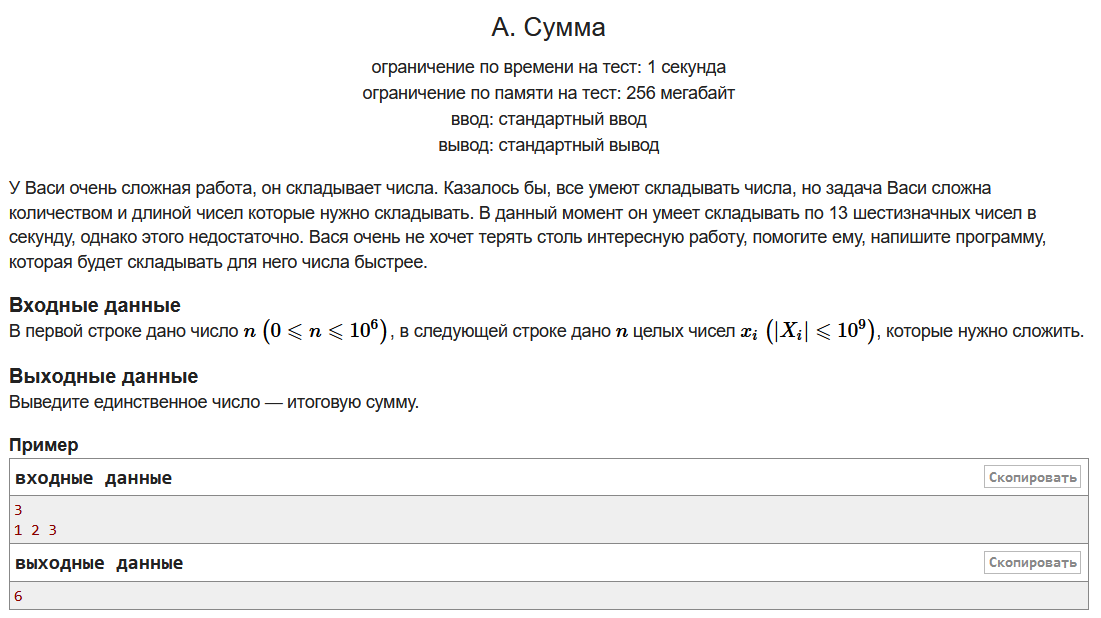
\includegraphics[width=\textwidth]{2A.png}
\end{center}
\subsubsection*{Идея решения}
Сначала заведем массив чисел и введем его через консоль с помощью цикла. Потом так же с помощью цикла просуммируем все числа в массиве и выведем ответ.
\subsubsection*{Исходный код}
\begin{lstlisting}
#include <iostream>
#include <string>
#include <unordered_map>
#include <unordered_set>
#include <algorithm>
#include <vector>
#include <cmath>
#include <iomanip>
using namespace std;
typedef long long ll;
int main()
{
	ios_base::sync_with_stdio(false);
	cin.tie(0);
	cout.tie(0);
	int n;
	cin >> n;
	ll ans = 0;
	for (int i = 0; i < n; i++) {
		ll x;
		cin >> x;
		ans += x;
	}
	cout << ans;
	return 0;
}
\end{lstlisting}
\subsubsection*{Фрагмент турнирной таблицы контеста}
\begin{center}
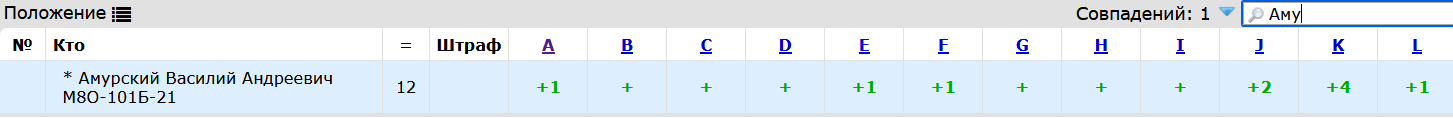
\includegraphics[width=\textwidth]{state2.png}\newline\noindent
\end{center}

\subsubsection*{Выводы}
Задача дорешана. Основные события отладки: неправильный ответ на претесте 1, забыл считать кол-во элементов в массиве.
